\documentclass[12pt]{exam}
\usepackage{xkcdcolors}
\usepackage{tikz}
\usetikzlibrary {intersections,calc,through,angles,quotes}

\newsavebox{\mysolution}

\newenvironment{blanksolution}
  {%
    \begin{lrbox}{\mysolution}%
    \begin{minipage}{\linewidth}%
  }
  {%
    \end{minipage}%
    \end{lrbox}%
    \ifprintanswers
      \usebox{\mysolution}%
    \else
      \vspace{\dimexpr\ht\mysolution+\dp\mysolution\relax}%
    \fi
  }
\begin{document}
\begin{questions}
    \question Construct the locus of points that are at a distance equal to the length of the given line segment $a$ from the given point $P$.

    \begin{tikzpicture}
        \draw[very thick,xkcdPurple] (0,0) -- node[midway,below] {$a$} (5,0);
        \node [fill=xkcdRed,inner sep=1pt,label=45:$P$] at (11,0) {};
    \begin{blanksolution}
        \draw (11,0) circle [radius=5];
    \end{blanksolution}
    \end{tikzpicture}

    \question Construct the locus of points that are at a the distance equal to the length of the given line segment $a$ from the given line $b$.

        \begin{tikzpicture}
        \draw[very thick,xkcdPurple,name path=l] (0,0) -- node[midway,below] {$a$} (0.8\textwidth,0);
        \draw[very thick,xkcdGreen] (0,4) -- node[midway,below] {$b$} (3,4);
        % \coordinate (A) at (4,0);
        % \begin{blanksolution}
        % \draw[name path=p] (A) circle [radius=1];
        % \fill [xkcdRed, opacity=0.5, name intersections={of=l and p, by = {A1,A2}}]
        %     (A1) circle (2pt) node {}
        %     (A2) circle (2pt) node {};
        % \draw[name path=ql] (A1) circle [radius=3];
        % \draw[name path=qr] (A2) circle [radius=3];
        % \fill [xkcdRed, opacity=0.5, name intersections={of=ql and qr, by = {B1,B2}}]
        %     (B1) circle (2pt) node {}
        %     (B2) circle (2pt) node {};
        % \draw ($(A)!2!(B2)$) -- ($(A)!2!(B1)$);
        % \draw[name path=r] (A) circle [radius=3];

        % \end{blanksolution}
    \end{tikzpicture}
    \newpage
    \question Construct the locus of points that are equidistant from the two given points.

    \vspace{0.1\textheight}
    \begin{center}
    \begin{tikzpicture}
                \node [fill=xkcdRed,inner sep=1pt,label=90:$P$] at (0,0) {};
                \node [fill=xkcdRed,inner sep=1pt,label=90:$Q$] at (6,1) {};
    \end{tikzpicture}
\end{center}
    \vspace{0.2\textheight}

    \question Construct the locus of points that are equidistant from the two given parallel lines.

    \vspace{0.1\textheight}
    \begin{center}
    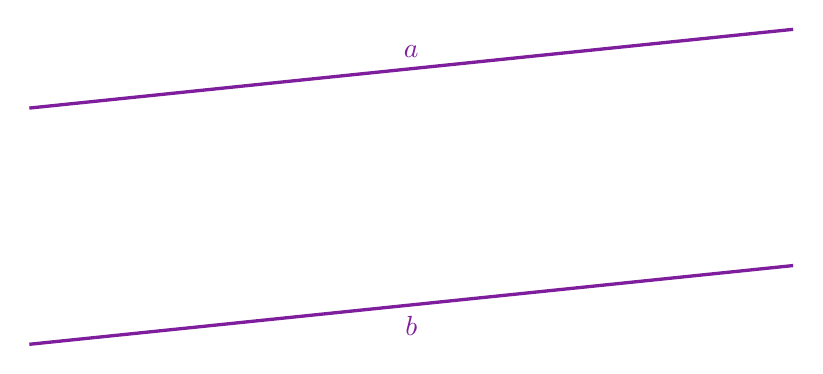
\begin{tikzpicture}
 \draw[very thick,xkcdPurple] (0,0) -- node[midway,below] {$b$} (0.8\textwidth,1);
  \draw[very thick,xkcdPurple,yshift=3cm] (0,0) -- node[midway,above] {$a$} (0.8\textwidth,1); 
    \end{tikzpicture}
\end{center}
    \vspace{0.2\textheight}
    \question Construct the locus of points that are equidistant from the two given intersecting lines.
    \vspace{0.1\textheight}
    \begin{center}
    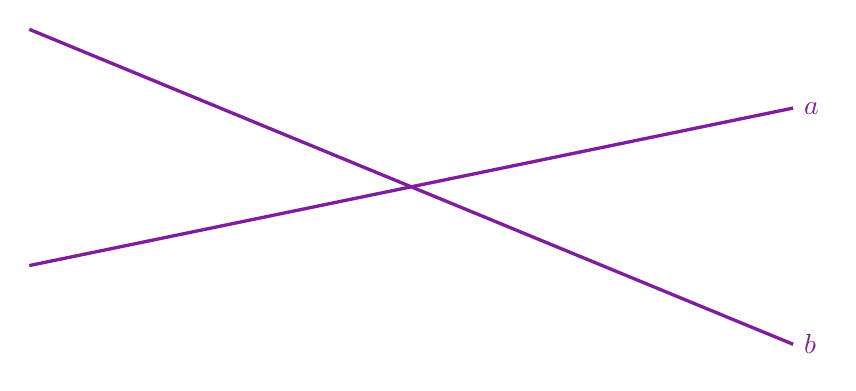
\begin{tikzpicture}
 \draw[very thick,xkcdPurple] (0,3) -- (0.8\textwidth,-1) node[right] {$b$} ;
  \draw[very thick,xkcdPurple] (0,0) -- (0.8\textwidth,2) node[right] {$a$} ; 
    \end{tikzpicture}
\end{center}
    \vspace{0.2\textheight}
    \question Construct a triangle whose sides have the following lengths.

    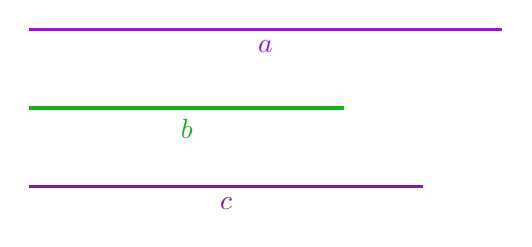
\begin{tikzpicture}
        \draw[very thick,xkcdPurple] (0,0) -- node[midway,below] {$c$} (5,0);
        \draw[very thick,xkcdGreen,yshift=1cm] (0,0) -- node[midway,below] {$b$} (4,0);
        \draw[very thick,xkcdViolet,yshift=2cm] (0,0) -- node[midway,below] {$a$} (6,0);
    \end{tikzpicture}
    \begin{parts}
        \part unknown:
        \begin{blanksolution}
            triangle
        \end{blanksolution}
        \part data:
          \begin{blanksolution}
            length of sides
        \end{blanksolution}
    \end{parts}

    \begin{blanksolution}
        \begin{tikzpicture}
            \coordinate [label=left:$B$] (B) at (0,0);
            \coordinate [label=right:$C$] (C) at (6,0);
            \draw[very thick,xkcdViolet] (B) -- node[midway,below] {$a$} (C);
            \draw[xkcdPurple,name path=c] (B) circle [radius=5];
            \draw[xkcdGreen,name path=b] (C) circle [radius=4];
            \fill [xkcdRed, opacity=0.5, name intersections={of=c and b, by = {A1,A2}}]
            (A1) circle (2pt) node {1}
            (A2) circle (2pt) node {2};
            \draw[very thick,xkcdPurple] (A1) -- (B) -- (A2);
            \draw[very thick,xkcdGreen] (A1) -- (C) -- (A2);
    \end{tikzpicture}
    \end{blanksolution}
\question Given a fixed line segment $AB$ and a fixed angle $\angle C$, construct the locus of points $C$ such that $\angle ACB$ is equal to the given angle.
    \vspace{0.1\textheight}
    \begin{center}
    \begin{tikzpicture}
        \coordinate [label=left:$A$] (A) at (0,0);
        \coordinate [label=right:$B$] (B) at (4.5,0);
        \draw[very thick] (A) -- (B);
        \coordinate (C) at (10,0);

        \draw (C)++(2,0) arc [start angle=0,end angle=40,radius=2];
        \draw (C) --++(0:3);
        \draw (C) --++(90:3);
        \draw (C) --++(40:3);

        \node[right] at ($(C)+(20:2)$) {$\angle C$};
    \end{tikzpicture}
\end{center}
    \vspace{0.2\textheight}
\end{questions}

\end{document}
\question Construct the perpendicular bisector of the line given below

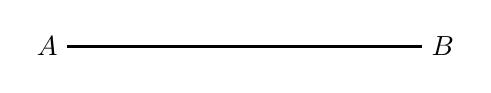
\begin{tikzpicture}
        \coordinate [label=left:$A$] (A) at (0,0);
        \coordinate [label=right:$B$] (B) at (4.5,0);
        \draw[very thick] (A) -- (B);
\end{tikzpicture}
\begin{parts}
        \part unknown:
        \begin{blanksolution}
           $CE$, the perpendicular bisector of $AB$
        \end{blanksolution}
        \part data:
          \begin{blanksolution}
            points $A$ and $B$
        \end{blanksolution}
        \part condition:
        \begin{blanksolution}
            $AD = DB$ and $CE \perp AB$ 
        \end{blanksolution}
    \end{parts}
    \begin{solution}
        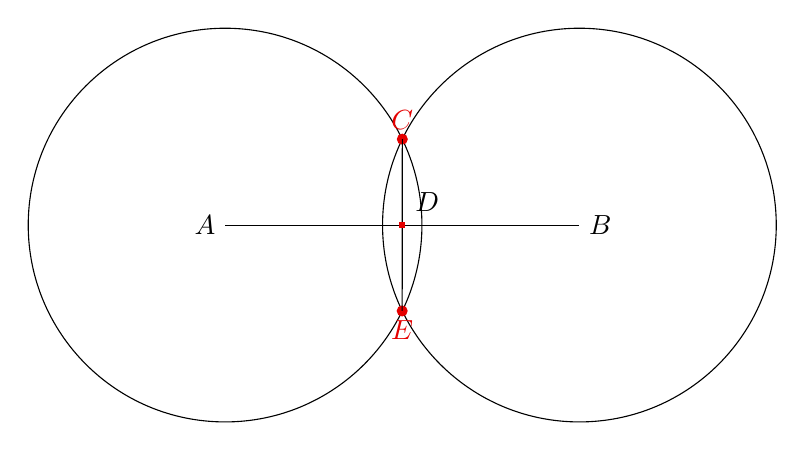
\begin{tikzpicture}
        \coordinate [label=left:$A$] (A) at (0,0);
        \coordinate [label=right:$B$] (B) at (4.5,0);
        \draw[name path=A--B] (A) -- (B);

        \draw[name path=r] (B) circle [radius=2.5];
        \draw[name path=l] (A) circle [radius=2.5];

        \fill [xkcdRed,name intersections={of=r and l, by = {[label=90:$C$]C,[label=-90:$E$]E}}] 
        (C) circle (2pt)
        (E) circle (2pt);

        \draw [name path=C--E] (C) -- (E);
        \path [name intersections={of=A--B and C--E,by=D}];
        \node [fill=xkcdRed,inner sep=1pt,label=45:$D$] at (D) {};
\end{tikzpicture}
    \end{solution}

\question Circumscribe a circle about the triangle given below

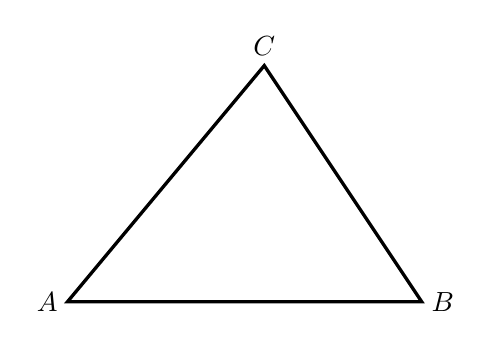
\begin{tikzpicture}
        \coordinate [label=left:$A$] (A) at (0,0);
        \coordinate [label=right:$B$] (B) at (4.5,0);
        \coordinate [label=above:$C$] (C) at (2.5,3);
        \draw[very thick] (A) -- (B) -- (C) -- cycle;
    \end{tikzpicture}
    \begin{parts}
        \part unknown:
        \begin{blanksolution}
            $X$ the centre of the Circle
        \end{blanksolution}
        \part data:
          \begin{blanksolution}
            points $A$, $B$, and $C$
        \end{blanksolution}
        \part condition:
        \begin{blanksolution}
            $XA=XB=XC$
        \end{blanksolution}
    \end{parts}

    \begin{blanksolution}
        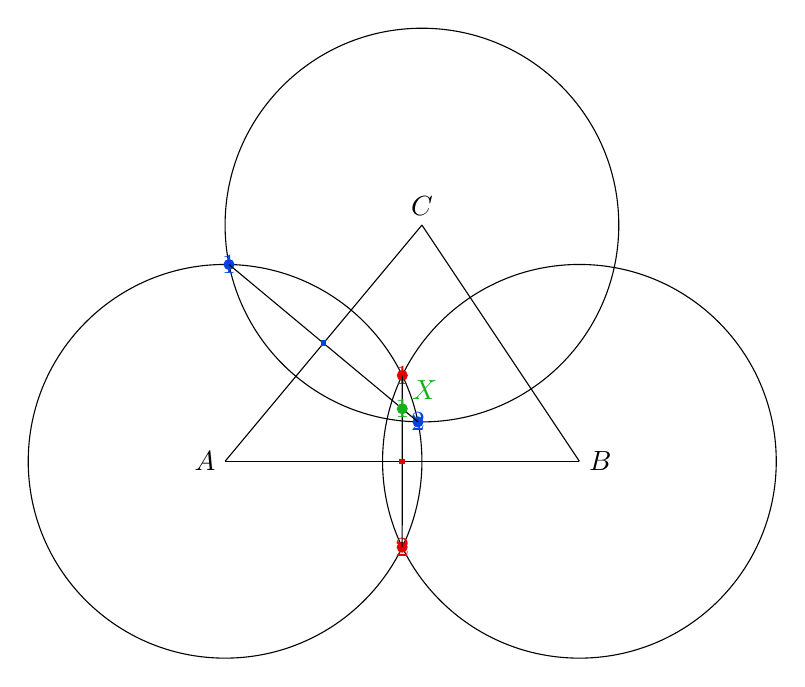
\begin{tikzpicture}
        \coordinate [label=left:$A$] (A) at (0,0);
        \coordinate [label=right:$B$] (B) at (4.5,0);
        \coordinate [label=above:$C$] (C) at (2.5,3);
        \draw[name path=A--B] (A) -- (B);
        \draw (B) -- (C);
        \draw[name path=A--C] (A) -- (C);

        \draw[name path=r] (B) circle [radius=2.5];
        \draw[name path=l] (A) circle [radius=2.5];
        \fill [xkcdRed,name intersections={of=r and l, by = {C1,C2}}] 
        (C1) circle (2pt) node {1}
        (C2) circle (2pt) node {2};

        \draw [name path=C1--C2] (C1) -- (C2);
        \path [name intersections={of=A--B and C1--C2,by=D}];
        \node [fill=xkcdRed,inner sep=1pt] at (D) {};

        \draw[name path=t] (C) circle [radius=2.5];
        \fill [xkcdBlue,name intersections={of=l and t, by = {B1,B2}}] 
        (B1) circle (2pt) node {1}
        (B2) circle (2pt) node {2};

        \draw [name path=B1--B2] (B1) -- (B2);
        \path [name intersections={of=A--C and B1--B2,by=E}];
        \node [fill=xkcdBlue,inner sep=1pt] at (E) {};

        \fill [xkcdGreen,name intersections={of=B1--B2 and C1--C2, by = {[label=45:$X$]X}}] 
        (X) circle (2pt) node {1};
    \end{tikzpicture}

    \end{blanksolution}
    \question Find the locus of points that are equidistant from two given lines.

    \question Inscribe a circle in the triangle given below

    \begin{tikzpicture}
        \coordinate [label=left:$A$] (A) at (0,0);
        \coordinate [label=right:$B$] (B) at (8.5,0);
        \coordinate [label=above:$C$] (C) at (4,5);
        \draw[very thick] (A) -- node[midway, below] {$c$} (B) -- node[midway, right] {$a$} (C) -- node[midway, left] {$b$} cycle;
    \end{tikzpicture}

    \begin{parts}
        \part unknown:
        \begin{blanksolution}
            $X$ the centre of the Circle
        \end{blanksolution}
        \part data:
          \begin{blanksolution}
            lines $a$, $b$, and $c$
        \end{blanksolution}
        \part condition:
        \begin{blanksolution}
            $X$ is at the same distance from lines $a$, $b$, and $c$
        \end{blanksolution}
    \end{parts}

So this exercise is mainly going to be to help you understand problem solving

Problem describe, or let's construct a triangle being given its three sides

So what I want you to do first is list all the given as in what is noon. Okay as in like if there is no known if there is no unknown, then we don't have to like there is no problem to solve right so in this problem, the unknown is the geometry figure, which is the right triangle so we are going to call the given as the data and what's the data we have for the first question, I'm going to give you all the three sides, the value of all the three sides, so the sheet you have three lines